\paragraph{Saturation bias}

\noindent
\begin{minipage}{\textwidth}
\includegraphics[width=0.3\linewidth]{src/figures/brighton.jpeg}
\hfill
\includegraphics[width=0.3\linewidth]{src/figures/brighton.jpeg}
\hfill
\includegraphics[width=0.3\linewidth]{src/figures/brighton.jpeg}

\captionof{figure}{\textbf{Lorem.} Ipsum!}
\end{minipage}


\begin{center}
    %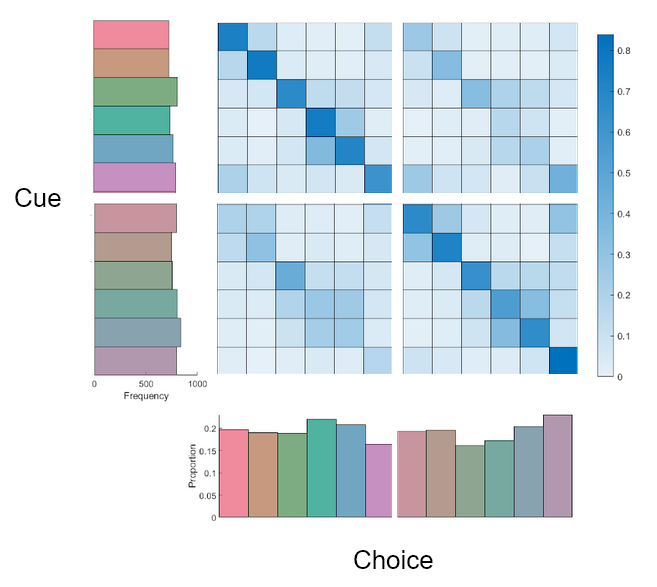
\includegraphics[width=\textwidth]{../../Figures/saturationBias.png}
    \includesvg[inkscapelatex=false, width=\textwidth]{../../Figures/working/Poster_components/Saturation copy.svg}
    \captionof{figure}{\textbf{Saturation Bias.}
    Heatmap of cues and corresponding choices. Selections along the negative diagonal correspond to correct choices. Choices along the negative diagonal in the bottom left and top right quadrants show trials on which an incorrect choice was made in such a way that the hue was correct but the higher or lower saturation versions of the cue were chosen (respectively). Note: the main diagonal is expected to be filled in at a greater extent regardless of performance level since the correct choice is shown on every trial, whereas only a subset of the incorrect choices are shown.}
    \label{fig:saturationBias}
\end{center}

Non-uniformities in CIELUV may also plausibly result in our nominally iso-saturated colors actually being variably saturated. This would be a concern, as it would be a reasonable prediction that higher saturation colors would be more salient, and thus more likely to be selected as responses. We see no (or very little) bias towards higher saturation colors in a control experiment. In \autoref{fig:saturationBias} it can be seen that there are a reasonable number of errors where an animal picks a higher saturation version of the same hue (lower left quadrant). Still, it is also seen that the number of errors of the inverse type (upper right quadrant) is roughly equal in number.

